\documentclass[a4paper,11pt]{article}

\usepackage{amsmath,amssymb,amsfonts,amsthm}    % Typical maths resource packages
\usepackage{graphicx}  
                        % Packages to allow inclusion of graphics
\usepackage{hyperref}                           % For creating hyperlinks in cross references
\usepackage[authoryear]{natbib}                 % literature reference style
\usepackage[bf]{caption2}
\usepackage{listings}
\usepackage{xcolor}  
\definecolor{dkgreen}{rgb}{0,0.6,0}
\definecolor{gray}{rgb}{0.5,0.5,0.5}
\definecolor{mauve}{rgb}{0.58,0,0.82}
\definecolor{lightgray}{gray}{0.95}
\lstset{language=R}
\lstset{breaklines}
\lstset{numbers=left,
	firstnumber = 1,
	backgroundcolor = \color{lightgray},
	numberstyle=\tiny\ttfamily,
	numbersep=5pt,
	numberblanklines=false,
	breaklines=true,
	showstringspaces=false,
	showspaces=false,
	frame=l,
	xleftmargin=5pt,
	xrightmargin=5pt,
	basicstyle=\ttfamily\scriptsize,
	stepnumber=1,
	keywordstyle=\color{blue},          
	commentstyle=\color{dkgreen},       
	stringstyle=\color{mauve}         
}  


% -------------------------------
% --- some layout definitions ---
% -------------------------------

% define topline
\usepackage[automark]{scrpage2}
\pagestyle{scrheadings}
\automark{section}
\clearscrheadings
\ohead{\headmark}

% define citation style
\bibliographystyle{ecta}

% define page size, margin size
\setlength{\headheight}{1.1\baselineskip}
\voffset=-2cm
\hoffset=-3cm
\textheight24cm
\textwidth15.5cm
\topmargin1cm
\oddsidemargin3cm
\evensidemargin3cm

% define line line spacing = 1.5
\renewcommand{\baselinestretch}{1.5}

% define second level for `itemizing'
\renewcommand{\labelitemii}{-}

\begin{document}
	\thispagestyle{empty}
\begin{center}
	
	{\Large{\bf Using Mechine Learning to Predict the Default Risk \\of Credit Card}} \vspace{0.5cm}
	
	
	{\normalsize A Student Project Report of \\Statistical Programming Language(SS-17) submitted\\\vspace{0.5cm}
		to}\\\vspace{0.5cm}
	{\normalsize{\bf Shi Chen\\
			Alla Petukhina\\
			Niels Wesselh\"offt
	}} \\\vspace{0.5cm}
	{\normalsize Ladislaus von Bortkiewicz Chair of Statistics\\
		C.A.S.E. – Center for Applied Statistics and Economics\\
		Humboldt-Universit\"at zu Berlin
	} \vspace{1cm}
	
	
	{\normalsize by \\\vspace{0.5cm}
		{\bf Jingmin Zhang(578516)\\
			Yiying Zhang(524900)} \\
	} \vspace{1cm}
	
	
	{\normalsize 
		Berlin, August 17, 2017}
	
\end{center}

\newpage
\tableofcontents
\clearpage

\newpage
\pagestyle{plain}
\setcounter{page}{1}    % start page numbering anew
\pagenumbering{arabic}  % page numbers in arabic style

\section{Introduction}
 In recent years, more and more people can get their credit card easily as the economics growing. Meanwhile, the default problem of the credit card is becoming more seriously.Many banks in world are all facing a problem about credit risk from their customers. On the one hand, banks are likely to make their requirements loose to attract new customers in this more and more competitive situation, on the other hand, they are afraid that their customers would lose their promises, thus it will induce them into bad situation, for instance, go bankruptcy. Therefore, predictions of their customer’s default payment in the future is essential for every bank by using statistical techniques, especially important for their risk management department. 
 
In fact, researchers used statistical methods for risk prediction in early 1997, like logistic regression according to \cite{Hand97Henley}. With the development of computer and machine learning, more methods were employed, for instance, neural network and random forests according to \cite{thomas2000} \cite{KH2002}. 

In this paper, we simulate the work of \cite{Cheng2009the} and try to prove their conclusion in our own way. The dataset that we used to construct our models is same, but the content of paper is different from pre-processing, building models and comparing results. However, we both has the same aim, which is to predict the probability of default payment as precisely as we can. 

In our assignment, we use Logistic Regression, Naive Bayes, Neural Network, Random Forest and Decision Trees to predict the probability of default payment. At last, we compared the AUC and accuracy of these models. We try to tackle this problem in our way and solve it. 

This paper is constructed as follows. Section one is theory and design, which includes 
theorems about handling outliers, models involved in the report and model performance evaluation. In section 2, data pre-processing and implementation of models are explained with main codes and figures. Section 3 is about empirical study, in the part, we focus on the dataset we employed, data visualization and results explanations of models, for instance, ROC curves comparison between models. The last part is our conclusion, where we provide our idea and thinking after our study

\newpage
\section{Theory and Design}
\subsection{Data Preprocessing}
\subsubsection{Handling Outliers}
Outliers are observations which deviate much from other observations in the dataset, and are regard as some mistakes or generated by a different mechanism.\cite{hawkins1980identification}They appear because of human error, instrument reading error and some deviation in populations. Outliers detection is one of the most important steps in machine learning since they behave differently from the norm and will influence the performance of prediction models. To improve the accuracy of our models, we need to remove or deal with those outliers separately.

In our project, the primary approach we used to detect the outliers is an unsupervised K-means clustering algorithm.\cite{loureiro2004outlier} Clustering algorithm aims to group the observations based on the similarity, this approach used clustering to find observations that are significantly different from the majority of the data and is more efficient. 

The k-means algorithm is used to partition a given set of observations into a predefined amount of $k$ clusters. The algorithm as described by \cite{macqueen1967some} starts with a random set of $k$ center-points ($\mu$). During each update step, all observations $x$ are assigned to their nearest center-point (see equation \ref{eqn:kmeans_assign_step}). 

\begin{equation}
S_i^{(t)} = \big \{ x_p : \big \| x_p - \mu^{(t)}_i \big \|^2 \le \big \| x_p - \mu^{(t)}_j \big \|^2 \ \forall j, 1 \le j \le k \big\}
\label{eqn:kmeans_assign_step}
\end{equation}

\subsection{Prediction Models}
\subsubsection{Logit Regression Model}
Generally, when researchers try to figure out the impact of variables on the probability of a specific event to occur, logistic regression often be used. Logistic regression has two types characterized by the number of categories of the dependent variable, binary logistic regression (2 categories) and multinomial logistic regression (n categories).

The technique of logistic regression is easy to understand with the basic knowledge of ordinary least square (OLS) due to their same general principles. The most important difference between these two regression models, which should be prior explain, is the type of the outcome variable. Specifically, the outcome variable of the logistic regression model is binary and dichotomous, but in OLS, where the outcome variable is assumed to be continuous (\cite{appliedlogit}).

The principles of logistic regression can be summarized as following. Firstly, building the logistic regression model and coding the dependent variable with the value of “0” and “1” (for binary logistic regression), respectively, are very necessary. Then, because the logistic model is non-linear and parameters can be estimated by maximum likelihood. After that, the value of parameters can be calculated, and the significance of these parameters can be concluded easily by using computer. 

\subsubsection{Naive Bayes Model}
Naive Bayes is based on Bayes theory and assumes that features are independent given class, which means,
\begin{equation}
P(X|C)=\prod_{i=1}^{n}P(X_{i}|C)
\end{equation}
\begin{equation}
X=\left ( x_{1},x_{2},...x_{n} \right )
\end{equation}
which represents some n features and C means a class. There are more details of this equation above as following.
Basing on Bayes theorem, the conditional probability can be written as:
\begin{equation}
p\left ( C_{k}|x \right )=\frac{p\left ( C_{k} \right )p\left ( x|C_{k} \right )}{p\left ( x \right )}
\end{equation}
We are focusing only on numerator of a fraction due to the independence of the denominator of C, therefore, using the chain rule in probability theory, the numerator can be written as follows,
\begin{equation}
p\left ( C_{k},x_{1},...,x_{n}\right )=p\left ( x_{1}|x_{2},...,x_{n},C_{k} \right )p\left ( x_{2}|x_{3},...,x_{n},C_{k} \right )...p\left ( x_{n-1}|x_{n},C_{k} \right )p\left ( x_{n}|C_{k} \right )p\left ( C_{k} \right )
\end{equation}
Now, the process of getting this equation is finishing and constructing a classifier from probability model can be done the next.As we all known, this assumption is unrealistic, however, the naïve Bayes is quite useful in practice world and especially in many complex situations. Another strong advantage of NB is that in practice it often competes well with more sophisticated classifiers (\cite{Rishnb}).

\subsubsection{Decision Trees Model}
Decision trees model is one of the basic algorithm in machine learning, it can be used both for classification and regression. Classification and regression trees (CART) algorithm can generate binary recursive partitioning procedure and is able to handle continuous and nominal attributes as dependent and independent variables (\cite{steinberg2009cart}). The model choose attributes which have best performance in distinguishing aimed groups. Every node of the trees denote a test of attributes and CART work by separate the data into smaller and homogeneous groups.  For a binary (0/1) target, the measure of homogeneity is Gini index, of a node x, the Gini index is calculated by equation \ref{eqn:Gini_Index}:
\begin{equation}
G(x)=1-p(x)^{2}+(1-p(x))^{2}
\label{eqn:Gini_Index}
\end{equation}
where p(x) is the (possibly weighted) relative frequency of class 1 in the node. The recursive procedure will stop until the pre-defined maximum depth or minimum number of observations in each node is reached.\\

\subsubsection{Random Forest Model}
Random forest belongs to the ensemble learning that contains many classification method and aggregate all of the results.Breiman \cite{breiman2001random} develop this algorithm as an extension of an ensemble of trees, and changed the way of constructing each classification trees. 

According to Breiman,\cite{breiman2001random} each node of random forest splits using the best among a subset of randomly chosen predictors at that node. This random selection of attributes at each node decreases the correlation between the trees in the forest and reduce the error rate. As a consequence, it allows random forest to outperform some other algorithm like logistic regression models\citealp{peters2004predictive} and ease the problem of overfitting. Besides, random forest also provide measures of the importance of each predictor variables\cite{breiman2001random}.we will discuss the variable importance in section 3 in detail.

The general algorithm of random forest can be stated as follow:
\begin{itemize}
	\item For n = 1 to n, set n bootstrap samples from the original data. For each of the bootstrap samples, grow an unpruned classification tree. 
	\item At each node, randomly sample x of the predictors and choose the best split among those variables.
	\item  Use model stopping criteria to determine when a tree is complete. (e.g. maximum number of trees)
	\item Predict new data by aggregating the predictions of the trees using majority votes for classification.
\end{itemize}

In random forest, it provides a measurement of importance of predictor variables. Random forest algorithm estimates the importance of a variable by looking at how much prediction error changes when out-of-bag (OOB) data for that variable is permuted while all others remained unchanged \cite{archer2008empirical}. The calculation is carried out one tree after another and calculates over all trees during the construction of random forest. The goal of this is to identify the most valuable variables that influent the performance of the model.

\subsubsection{Neural Network}
The neural network is a mathematical model which based on human brain’s activity that can tackle both complex problems of classification and regression. Human brain is composed of around 10 million cells called neurons, each of them connected to other neurons to transmit information. In the neural network, instead of neurons in our brains, many artificial neurons work as biological one. 
Typically, neurons are grouped into layers. In general, there are three layers in neural network called input, hidden and output (\cite{NN97}). Of course, different layers have different functions in processing the signal.
 \begin{figure}[!ht] 
	\centering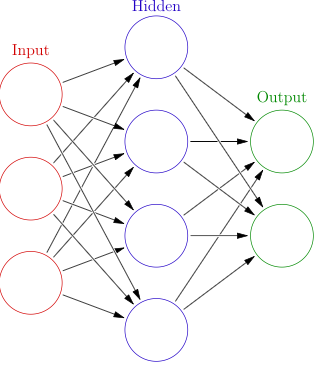
\includegraphics[width=3in]{Figures/NN} 
	\caption{Three layers of Neural Network \protect\includegraphics[scale=0.1]{Figures/qletlogo.pdf}\href{https://github.com/Jingmin24/R-programming/tree/master/SPL_Report}{SPL\_Report}}\label{fig:NN} 
\end{figure}

\subsection{Model Evaluation}
In order to have a more precise evaluation of our project, we use receiver operating characteristic (ROC) curve, which is a generalization of the confusion matrix, and the area under the ROC curve (AUC), which is a combined measure of sensitivity and specificity, to measure the overall accuracy of prediction models.\cite{bradley1997use}

The ROC curve shows the performance of a two class classifier across the range of possible predetermined threshold value, and plots test sensitivity along the y axis versus its 1-specificity along the x axis.\cite{park2004receiver} The perfect model will have an AUC value equals to 1.0 and a diagnostic test with an AUC value greater than 0.5 is better than relying on randomly assigned classifier.\\

\newpage
\section{Implementation}
\subsection{Data Preprocessing}
\subsubsection{Handling Outliers}
We will focus on the outliers handling approach in this subsection, in our dataset, we deal with outliers in categorical and numerical variables separately.

(1) Categorical variables\\
For variable ``Education (4 levels)" and ``Marriage (4 levels)" which described the situation of education and marriage of observation respectively, we used the most frequent value, mode, to replace the abnormal value which are not in data description.

(2) Continuous variables\\
Here we use k-means cluster to deal with continuous variables related to ``bill-statement" and ``payment" from month April to September,in total 12 variables. Because the method and code are almost same for these two groups of variables, we will only discuss how we deal with 6 bill-statement variables in detail.

\begin{lstlisting}[language=R]
DataBill=scale(data.frame(df$BILL_AMT1,df$BILL_AMT2,df$BILL_AMT3,df$BILL_AMT4,df$BILL_AMT5,df$BILL_AMT6))
set.seed(123)
k_evaluation<-c()
for(i in 1:10){
km=kmeans(DataBill,center=i,iter.max =100)
k_evaluation<-c(k_evaluation,km$betweenss/(km$tot.withinss+km$betweenss))
}
k=which.max(k_evaluation)
km=kmeans(DataBill,center=k,iter.max =100)
##calculate the distance#######
dist.Bill=c()
for(i in 1:k){
c0=matrix(km$centers[i,],nrow=30000, ncol =6 , byrow = T)  
dist.Bill= cbind(dist.Bill,sqrt(rowSums((DataBill-c0)^2)))
}
##find the minimum distance of each observation###
y=apply(dist.Bill, 1, min)  
upper.limit = quantile(y,.98)
plot(1:30000,y,xlim=c(0,30000),xlab="sampleBill",ylab="Euclidean distance")  
points(which(y>upper.limit),y[which(y>upper.limit)],pch=19,col="red")
df[which(y > upper.limit),13:18] = NA
\end{lstlisting}
In line 1, we fist build a data frame contains 6 variables related to bill-statement and standardize the numerical value, then use k-menas algorithm to cluster these variables. The function we used is ``kmeans". 

From line 2 to 7, we make a loop to set the number of cluster from 1 to 10 and evaluate the result for each number of total clusters by calculating within sum of squares (WSS) that measure the difference within cluster, and between sum of squares (BSS) that measure the difference between clusters. With lower WSS and higher BSS value, the cluster will have more convincible result. \cite{brun2007model} In line 8 to 9, we pick up the best performed cluster result. Then in line 12 to 15, we build another loop to calculate the Euclidean distance (given in equation  \ref{eqn:Euc_dist}) of each each observation to the 10 centers.
\begin{equation}
 d(p,q)=\sqrt{\sum\limits_{i=1}^{n}(p_i-q_i)^2}
\label{eqn:Euc_dist}
\end{equation}
Then in line 17 to 20, we set the observations which are separated from the main clustering center as outliers. The threshold we used is 0.98 quantile of the total dataset, we excluded observations whose minimum distance are larger than this value. After this step, we delete in total 893 observations, which are regarded as outliers.
 \begin{figure}[!ht] 
	\centering\includegraphics[width=4in]{Figures/samplebills.pdf} 
	\caption{Outliers in Variables Billstatement\protect\includegraphics[scale=0.1]{Figures/qletlogo.pdf}\href{https://github.com/Jingmin24/R-programming/tree/master/SPL_Datacleaning}{SPL\_DataCleaning}}\label{fig:samplebill} 
\end{figure}

Figure \ref{fig:samplebill} shows the result of this procedure, the red points here represent the outliers related to variables ``Billstatement", we can find that red points have significant bigger distance, after removing these observations, the dataset will more suitable for building the prediction models.
\subsubsection{Standardization and Creating Dummy Variables }
Besides the basic procedures for data cleaning, more need to be done to pre-process the dataset to increase the accuracy of prediction from models. In this assignment, considering characters of the dataset and types of variables, we run codes for data pre-processing as followings.Packages called ``dummies'' and ``data.table'' be library for changing some variables to dummy variable.
\begin{lstlisting}[language=R]
SEX.d<-dummy("SEX",data = clean.df.nn,fun = as.integer,verbose = FALSE)
EDU.d<-dummy("EDUCATION",data = clean.df.nn,fun = as.integer,verbose = FALSE)
MAR.d<-dummy("MARRIAGE",data = clean.df.nn,fun = as.integer,verbose = FALSE)
AGE.d<-dummy("AGE",data = clean.df.nn,fun = as.integer,verbose = FALSE)
P0.d<-dummy("PAY_0",data = clean.df.nn,fun = as.integer,verbose = FALSE)
\end{lstlisting}
Some examples are given above. By running line 1, the variable ``SEX'' can be translate into two dummy variables. ``SEX'' points out which variable will be processed in the object dataset and ``data'' indicates our object dataset. ``verbose'' is a logical argument which can be set either ``TURE'' of ``FLASE'', which means whether to print the number of dummy variables. Similarly, variables named ``EDUCATION'', ``MARRIAGE'', ``AGE'' and ``Bill Payment'' are changed to dummy by applying same function and setting almost similar arguments. 
\begin{lstlisting}[language=R]
clean.df.dumm<-data.table(clean.df.nn,SEX.d,EDU.d,MAR.d,AGE.d,P0.d,P2.d,P3.d,P4.d,P5.d,P6.d)
clean.df.dumm[,c(2:11)]<-NULL
\end{lstlisting}
In line 1 above, these new created dummy variables are combined with the original dataset. By running line 2, original variables are deleted in necessary, because new dummy variables are inputted in the model instead of old factor variables.
\begin{lstlisting}[language=R]
stan<-function(x){
mu<-mean(x)
std<-sd(x)
result.stan<-(x-mu)/std
return(result.stan)
}
clean.df.nn[,c(12:23)]<-lapply(clean.df.nn[,c(12:23)],stan)
\end{lstlisting}
For numeric variables, standardizing is essential for improving the accuracy. Function makes standardize simpler and easier, if numeric variables are more than one in the dataset. By setting a function and using the function named ``lapply'', all numeric variables in dataset named ``clean.df.nn'' can be standardized.
\subsubsection{Correlation Matrix}
\begin{lstlisting}[language=R]
install.packages("corrplot")
library(corrplot)
loans_numeric<-sapply(clean.df,is.numeric)
correlation<-cor(clean.df[,loans_numeric])
corrplot(correlation,type = "upper"
,tl.pos = "d",tl.col = "black",tl.cex = 0.6)
corrplot(correlation,add = TRUE,type = "lower",
method = "number",diag=FALSE
,tl.pos = "n",
cl.pos = "n",cl.ratio= 0.2,addCoefasPercent = TRUE)
\end{lstlisting}
Codes for getting this correlation matrix consists of two parts: at first, correlation matrix should be made by function ``cor''. In the second part, setting essential arguments with package ``corrplot'' to get a final correlation table.

In line 4 above, the report used ``cor'' function to calculate the correlation coefficient between these numeric variables in dataset named clean.df. After running this line 4 and line 5, a plain correlation matrix with numbers can be concluded. In line 6 and line 7, ``type'' denotes that this code is for construct the upper triangle. ``tl.pos'', ``tl.col'' and ``tl.cex'' denotes that the place, color and size of names of these variables. From line 8 to line 11, this code is used to construct the lower triangle by setting the argument ``type''. ``add=TRUE'' denotes that this lower triangle will be combined with the upper one. By setting ``tl.pos'', ``cl.pos'' and ``cl.ratio'', the size of the correlation coefficient in the lower triangle can be adjusted.

\subsection{Prediction Models}
Before building all the models, we first separate the data into train and test set by setting 80\% of the data to train the model and 20\% to test the result.
\begin{lstlisting}[language=R]
set.seed(1234)
idx.train <- createDataPartition(y = clean.df$default.payment.next.month, 
p = 0.8, list = FALSE) 
clean.df.train <- clean.df[idx.train, ] 
clean.df.test <-  clean.df[-idx.train, ] 
\end{lstlisting}
The function we used here is ``createDataPartition" from package ``caret". In line2, the target variable y is ``default.payment.next.month", and ``p=0.8" means the percentage of train set is 80\%.
\subsubsection{Logit Regression Model}
In our assignment, our goal is to build the logistic model to estimate the probabilities of default payment. After data processing, we use the ``default payment'' as our dependent variable and other variables as independent variables to build the logistic model. By constructing the correlation table, 5 ``Amount of bill payment'' variables have been deleted in the logit regression model due to their large correlation coefficients. 
\begin{lstlisting}[language=R]
lr<-glm(default.payment.next.month~.,data=train_lr,family = binomial(link="logit"))
pred.lr <- predict(lr, newdata = test_lr,type = "response")
round(coef(summary(lr)),4)
\end{lstlisting}
The code of logit regression model is simpler than constructing other models, because it is a basic and popular one. In line 1, ``glm'' function is employed to construct the model with variables in dataset ``train.lr''. Apparently, the dependent variable y is ``defaut.payment.next.month'', and ``$\sim$.'' means, other variables in the same dataset are as independent variables. In line 2, ``newdata'' denotes a new dataset used to test the model. In line 3, function ``round'' can keep four decimals of coefficients.

One of the advantages of logistic regression is that the probability of a binomial phenomenon under one specific situation can be estimated. And that is why the logistic regression works for our assignment. Another advantage of the logistic regression is user-friendly and easy to explain. Besides, comparing with random forest, the logistic regression is very sensitive to data, which is its disadvantage. Before building a logistic model, closely data processing is very necessary.
\subsubsection{Naive Bayes model}
\begin{lstlisting}[language=R]
install.packages("e1071")
library("e1071")
df_nb<-naiveBayes(train$default.payment.next.month~.,data=train)
pred.nb<-predict(df_nb,newdata = test,type = "raw")
test$pred.nb<-pred.nb[,2]
\end{lstlisting}
The code of applying Naive Bayes model in our assignment is quite simple. Package named ``e1071'' is in application by running the line 1 and line 2. In naiveBayes function from line 3, here we have some arguments, for instance, ``data'' decides that dataset called ``train'' would be used for constructing NB model, and variable named ``default. payment. next. month'' is y, however, other variables would be as explanatory variables in the model. In line 4, ``type = raw'' denotes that the conditional probabilities for each class are returned.Unlike other model, two columns of probabilities are computed after running line 4. In fact, we only need one columns, therefore, code in line 5 is necessary to leave the probability of default (1=Yes).

\subsubsection{Decision Trees Model}
In this section, we used a popular package ``rpart" to build the decision trees model. It can use Gini-index or information increase as metric to build the trees.
\begin{lstlisting}[language=R]
#use pruning to decrease the probability of overfitting of the model
rpart.control=rpart.control(minsplit = 6, minbucket = 6,
cp=0.001, xval = 5, maxdepth = 6)
#build the decision model#
dt<-rpart(default.payment.next.month ~ ., data = clean.df.train, 
parms = list(split = "Gini"), method="class", control = rpart.control)
##predict the test set
pred.dt <- predict(dt, newdata = clean.df.test, type = "prob")[, 2]
pred.dt.class <-as.matrix(factor(ifelse(pred.dt > 0.5, "good","default")))
\end{lstlisting}
If the tree become too big, it will increase the possibility of overfitting of the model, which will made the model perform poorly when implement in test data. So from line 2 to 3, with function ``rpart.control", we pre-pure the tree by setting some parameters to stop the tree grow beyond limit. ``minsplit" means the minimum number of observations that must exist in a node, ``cp" is a complexity parameter, we also conduct a test to find the optimal value, which is around 0.001, and ``maxdepth" is the maximum depth of any node of the final tree. From line 5 to 6, we build the tree model using function ``rpart", in order to have classification result, we set ``method" as ``class".The parameter parms represents the splitting metric. The splitting index can be ``Gini" or ``Information", both measure the impurity of each node.

The advantage of single decision tree is that it is easy to interpret, when looking at the structure of the classification tree, we can get information of the results of each test in the node and also the percentage of total observations being assign in both classes. In particular variables which are not showed in the tree had less or no contribution to the model compared to the previously chosen splitting variables.

\subsubsection{Random Forest Model}
In this section, we use package ``caret" and ``randomForest" together to build the random forest model.
\begin{lstlisting}[language=R]
##cross validation for the train dataset
set.seed(1234)
model.control <- trainControl(method = "cv", number = 5, classProbs = TRUE, summaryFunction = twoClassSummary, allowParallel = TRUE )
rf.parms <- expand.grid(mtry =1:10)
# Train model with a 3-fold cross validation 
rf.caret <- train(default.payment.next.month~., data = clean.df.train, importance = T, method = "rf", ntree = 500, tuneGrid = rf.parms, 
metric = "ROC", trControl = model.control)
# test the model with predict function#
pred.rf.caret   <- predict(rf.caret, newdata = clean.df.test, type = "prob")[,2]
threshold<-0.5
pred.rf.class <-as.matrix(factor(ifelse(pred.rf.caret > threshold, "good",  "default")))
\end{lstlisting}
Before building the model, in line 3, we first use function ``trainControl" to preset some parameters of cross-validation, ``cv" means the method is cross-validation, the number of folds of cross validation equals to 5. The goal of this step is to reduce overfitting of the model in training process.

In line 4, we use ``expand.grid" to find the optimal value in range 1 to 10 of ``mtry"(the number of variables used in each node) since the model is quiet sensible to this parameter. 
 \begin{figure}[!ht] 
	\centering\includegraphics[width=4in]{Figures/rfmtry.pdf} 
	\caption{Test of ``mtry" in Random Forest\protect\includegraphics[scale=0.1]{Figures/qletlogo.pdf}\href{https://github.com/Jingmin24/R-programming/tree/master/SPL_RandomForest}{SPL\_Randomforest}}\label{fig:rfmtry} 
\end{figure}\\
Figure \ref{fig:rfmtry} shows the result of the test. The y label represents the ROC metric of the model for the number of each ``mtry", we can see that the ROC has a trend of increasing when the number become bigger and the line reaches the maximum value when ``mtry" equals to 10. So we set ``mtry" equals to 10 to build the random forest model. 

Then In line 6, we build the model with function ``train()" in ``caret" package by setting the response variable as ``default.payment.next.month", and use all other variable as predictors, ``ntree" means the total number of trees grown and ``importance" is to help us check the importance of variables in random forest.

In line 9, we test the result by predicting outcome using data in test set, the outputs are the probability of each observation being in good/default class, we set the threshold equals to 0.5.

\begin{lstlisting}[language=R]
####another way to check the importance with fuction "randomforest"
library(randomForest)
rf.fit <- randomForest(default.payment.next.month~., data=clean.df.train, 
ntree = 500, nodesize = 5, mtry = 10) 
###make a plot of variable importance
varImpPlot(rf.fit, n.var = 20, scale = T,main = "Importance of Variables")
\end{lstlisting}
Here in lines 3 and 4, we build another random forest model using function ``randomForest" from package ``randomForest" with similar parameters as before, the advantage is that this package provides a better plot of variable importance. In line 6, function ``varImpPlot" can generate a plot with top 20 most important variable, ``scale= T" means we scale the result to make it more easily to compare.

 \begin{figure}[!ht] 
	\centering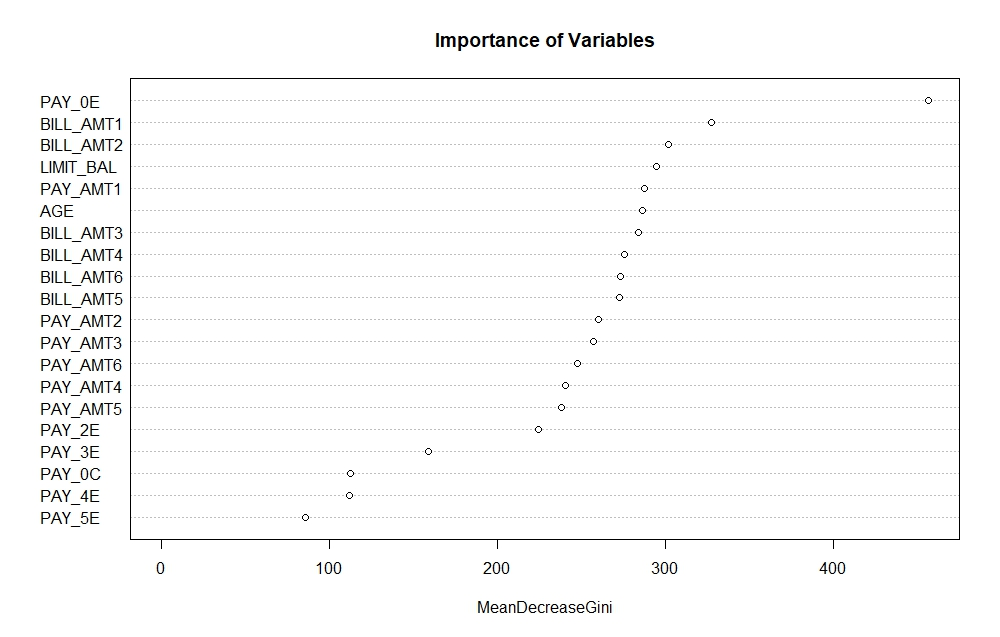
\includegraphics[width=4in]{Figures/VARimp.jpeg} 
	\caption{Variable Importance in Random Forest\protect\includegraphics[scale=0.1]{Figures/qletlogo.pdf}\href{https://github.com/Jingmin24/R-programming/tree/master/SPL_RandomForest}{SPL\_Randomforest}}\label{fig:rfimp} 
\end{figure}
Figure \ref{fig:rfimp} shows the results of top 20 most important variables of the random forests model. The measurement criteria is the mean decrease in Gini index when we set each variable randomly. We can see that the value of importance is scaled from 0 to 500. The most important variable is ``PAY\_0" which represents the pay-states in September, followed by variables related to the amount of bill-statement in previous months and the total amount of credit ``Limit\_Ball".

We can interpret from this results that the most recent credit situation is very important to predict the possibility of default in the future. A person who had default experience is more likely to default again. Age is also an influential factor, since in general, people in middle age will have large amount of wage and is less likely to default than younger generation. For variable ``Limit\_Ball", we also find that customers in ``good" class have higher amount of credit than ``default" class. Other attributes like bill-statement and payment in different months have similar level of influence on the prediction.    
\subsubsection{Neural Network}
\begin{lstlisting}[language=R]
clean.df.dumm.c<-clean.df.dumm[sample(1:nrow(clean.df.dumm),length(1:nrow(clean.df.dumm))),1:ncol(clean.df.dumm)]
Values<-clean.df.dumm.c[,c(1:13,15:90)]
Targets<-decodeClassLabels(clean.df.dumm.c$default.payment.next.month)
clean.df.dumm.c<-splitForTrainingAndTest(Values,Targets,ratio = 0.2)
clean.df.dumm.c<-normTrainingAndTestSet(clean.df.dumm.c)
model <- mlp(clean.df.dumm.c$inputsTrain, clean.df.dumm.c$targetsTrain, size=5, learnFuncParams=c(0.1), 
maxit=50, inputsTest=clean.df.dumm.c$inputsTest, targetsTest=clean.df.dumm.c$targetsTest)
prediction.nn<-predict(model,clean.df.dumm.c$inputsTest)
\end{lstlisting}
In fact, there are many packages in building neural network model, for example, ``nnet'', ``AMORE”
'' and ``neuralnet''. In our assignment, to build neural network model, packages named ``RSNNS'' is employed, which is a newer and more useful package. Besides, package ``Rcpp'' should be installed in this part in complement. In line 1, we upset the order of our dataset called ``clean.df.dumm''. In line 2 and line 3, ``Values'' and ``Targets'' are assigned values from the dataset and would be X and Y in the model.In line 4, the dataset is divided into two parts, one for building a model and anther for testing the model. In line 6, ``size'' denotes that there are 5 units in the hidden layers. By running line 7, prediction is concluded with the model we build above.

\subsection{Model Evaluation}
\begin{lstlisting}[language=R]
#check the confusion matrix and AUC#
confusionMatrix(pred.rf.class, clean.df.test$default.payment.next.month)
auc.caret <- auc(clean.df.test$default.payment.next.month, pred.rf.caret) 
########plot ROC curve together with the result from DTs
plot.roc(clean.df.test$default.payment.next.month, pred.rf.caret, 
print.auc=F,col="red")
\end{lstlisting}
We check the ROC curve and confusion matrix for each model, here we use the code in decision trees model as an instance. In line 2, we check the confision matrix, the positive class is ``default". In line 5, we use data in ``clean.df.text" as reference and plot the ROC curve of the model based on the confusion matrix.

\newpage
\section{Empirical Study}
\subsection{Data Description}
As a starting point of a predictive analysis it is necessary to understand the data which were inputted in our models. Data description assists us to get a deeper understanding of our data and variables, of course, the relationships between variables, which makes us easier to get conclusions and our results. Data visualization is essential because it will communicate information clearly and efficiently via graphics and plots, which will make complex data and the relationship between variables more understandable and useful for us. Therefore, in this part, appropriate method of data visualization was used to get a better idea of our dataset.

Basically, there are 24 variables in all and 23 of them are independent variables, the last one is a binary variable (Yes=1, No=0) as our dependent variable in the model. In this dataset, we have 30000 observations in total. More detailed description of these variables is as following. 

The first five variables are about some basic information of this credit card holder, which are ``the amount of given credit in all'', ``gender'', ``education'', ``marital status'' and ``age''. These variables are characters of this observation; it is necessary because some credit card holders with same character may have high default rate. From the 6th variable to the 11th variable, they represent the history of past payment from April to September, 2015. From -1 to 9, 10 different numbers are the measurement scale for different repayment status. From 12th variable to 17th variable, these were amount of bill payment during the same period above and their unit is dollar. The last six explanatory variables represent the amount of previous payment, which are in identical period and have same dollar unit. 

\begin{table}[ht]
	\begin{center}
		{\footnotesize
			\begin{tabular}{l|cc}
				\hline \hline
				& Information & \\
				\hline
				X1  & Amount of given credit(dollar), individual credit and his family credit  \\
				X2 & Gender (1=male, 2=female)  \\
				X3   &  Education (1=graduate school, 2=university, 3=high school, 4=others) \\
				X4    & Marital status (1=married, 2=single, 3=others)  \\
				X5   &  Age (year) \\
				X6-X11   & History of past payment (From April to September, 2005)  \\
				X12-X17   & Amount of Bill payment (dollar)\\
				X18-X23   & Amount of previous payment (dollar)  \\
				Y   &  Default payment (yes=1, no=0) \\
				\hline \hline
		\end{tabular}}
	\end{center}
	\caption{Information about variables}
\end{table}

\subsection{Data Visualization}
 \begin{figure}[!ht] 
	\centering\includegraphics[width=4in]{Figures/BillDiff.pdf} 
	\caption{Comparison of average value in variables ``Billstatement" with default and good class in credit stats\protect\includegraphics[scale=0.1]{Figures/qletlogo.pdf}\href{https://github.com/Jingmin24/R-programming/tree/master/SPL_DataVisualization}{SPL\_Datavisualization}}\label{fig:diffbill} 
	\centering\includegraphics[width=4in]{Figures/PaymentDiff.pdf} 
	\caption{Comparison of average value in variables ``payment" with default and good class in credit state\protect\includegraphics[scale=0.1]{Figures/qletlogo.pdf}\href{https://github.com/Jingmin24/R-programming/tree/master/SPL_DataVisualization}{SPL\_Datavisualization}}\label{fig:diffpay} 
\end{figure}
In the database, there are twelve variables related to bill-statement and payment from April to September, these variables have similar pattern and in order to have a clear impression of these variable, we visualize the difference of mean value of two classes in aimed variable ``default.payment.next.month".

We can see from figure \ref{fig:diffbill} and \ref{fig:diffpay}, customers who don`t default, which is the ``good" class in credit state, have higher amount of bill-statement and payment. Also for payment, there are significant lower average value of customer who default. Apart from that, with similar level of bill-statement in both classes, the average amounts of bill-statements are higher than the amounts of payments in ``default" class. This result suggests that, the customers with ``good" class in credit state normally have high ability to pay back to the bank. On the contrary, the ``default" class always use the money beyond their capability and fail to repay the credit card. It is necessary for bank to detect this kind of customers and avoid to give them large amount of credit.

Figure \ref{fig:Corr} shows a correlation matrix which was created with ``corrplot'' package. Correlation between each pair of numeric and dummy variables, excluding some factor variables. 

 \begin{figure}[!ht] 
	\centering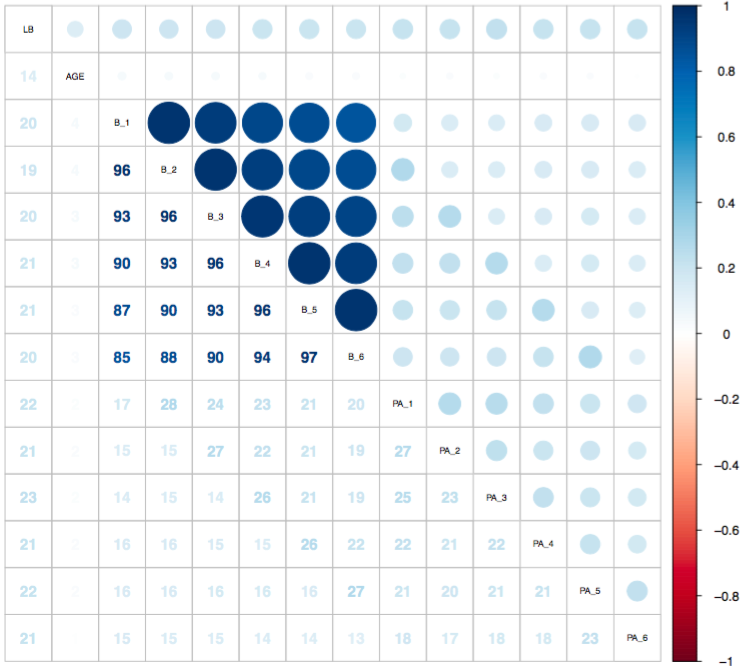
\includegraphics[width=5in]{Figures/Corr.png} 
	\caption{Correlation Table\protect\includegraphics[scale=0.1]{Figures/qletlogo.pdf}\href{https://github.com/Jingmin24/R-programming/tree/master/SPL_DataVisualization}{SPL\_DataVisualization}}\label{fig:Corr} 
\end{figure}
There are two symmetric triangles in this matrix. In the upper one, a dot-representation is used where blue dot represents positive correlation. No red dot means no negative correlation between attributes in our dataset. The size of the dot shows us the strong or weak relationship between these variables. The larger the dot, the stronger relationship they have. In the lower triangle, these numbers represent the correlation coefficients between these variables, which has the same meaning as symmetrical blue dot. Clearly, the correlation coefficients between ``Amount of bill payment'' variables are large enough to be eliminated in the logit regression model, in case of multicollinearity.
\subsection{Prediction Models}
In this section, we will discuss the input, expected and actual output of prediction models.
\subsubsection{Decision trees and random forest Models} 
\begin{itemize}
	\item Input
\end{itemize}
Since the decision trees and random forest models are both based on trees model and have some similarity in algorithm, we will discuss the empirical approach of these two models together.

The dataset we used to build these two models are based on the cleaned dataset after handling the outliers, after this step, we standardize all numerical variables and change all the categorical variables into dummy variables. We use Z-score to normalize numerical variable, the formula of z-score stated below in equation \ref{eqn:Z-score}:
\begin{equation}
Z=\frac{X-E(X)}{\sigma(X)}
\label{eqn:Z-score}
\end{equation}
After the standardization, all continuous variables can be compared under same metrics, positive and negative numbers represent higher and lower than average value respectively. This will make the data more easily to compare in the tree based models.

Besides, We also create new dummy variables of each level in categorical variables. Compared to categorical variables which have many values, two-class dummy variables can reduce the difficulty of searching the best categorical split to node. Particularly in random forest implementation, the computation for categorical variable in only related to the random selection of subsets of the category.\cite{breiman2001random} So this will also increase the accuracy of the prediction results. After this transformation, we have 88 variables in the cleaned dataset.

Then we build the classification trees and random forest model of response variable setting as ``default.payment.next.month" on the train set with five-fold cross validations. And test the models based on test set, the threshold of distinction of probability is set as 0.5.
\begin{itemize}
	\item Expected output
\end{itemize}
For decision trees model, we expect to get a plot showing the process of how the tree are grown, each node denote good/default classification with predicted probability. Since random forest model is more robust than decision trees and has less likely of overfitting, it may yield better results.
\begin{itemize}
	\item Actual output
\end{itemize}
For decision trees model, we visualize the tree with function ``prp".
 \begin{figure}[!ht] 
	\centering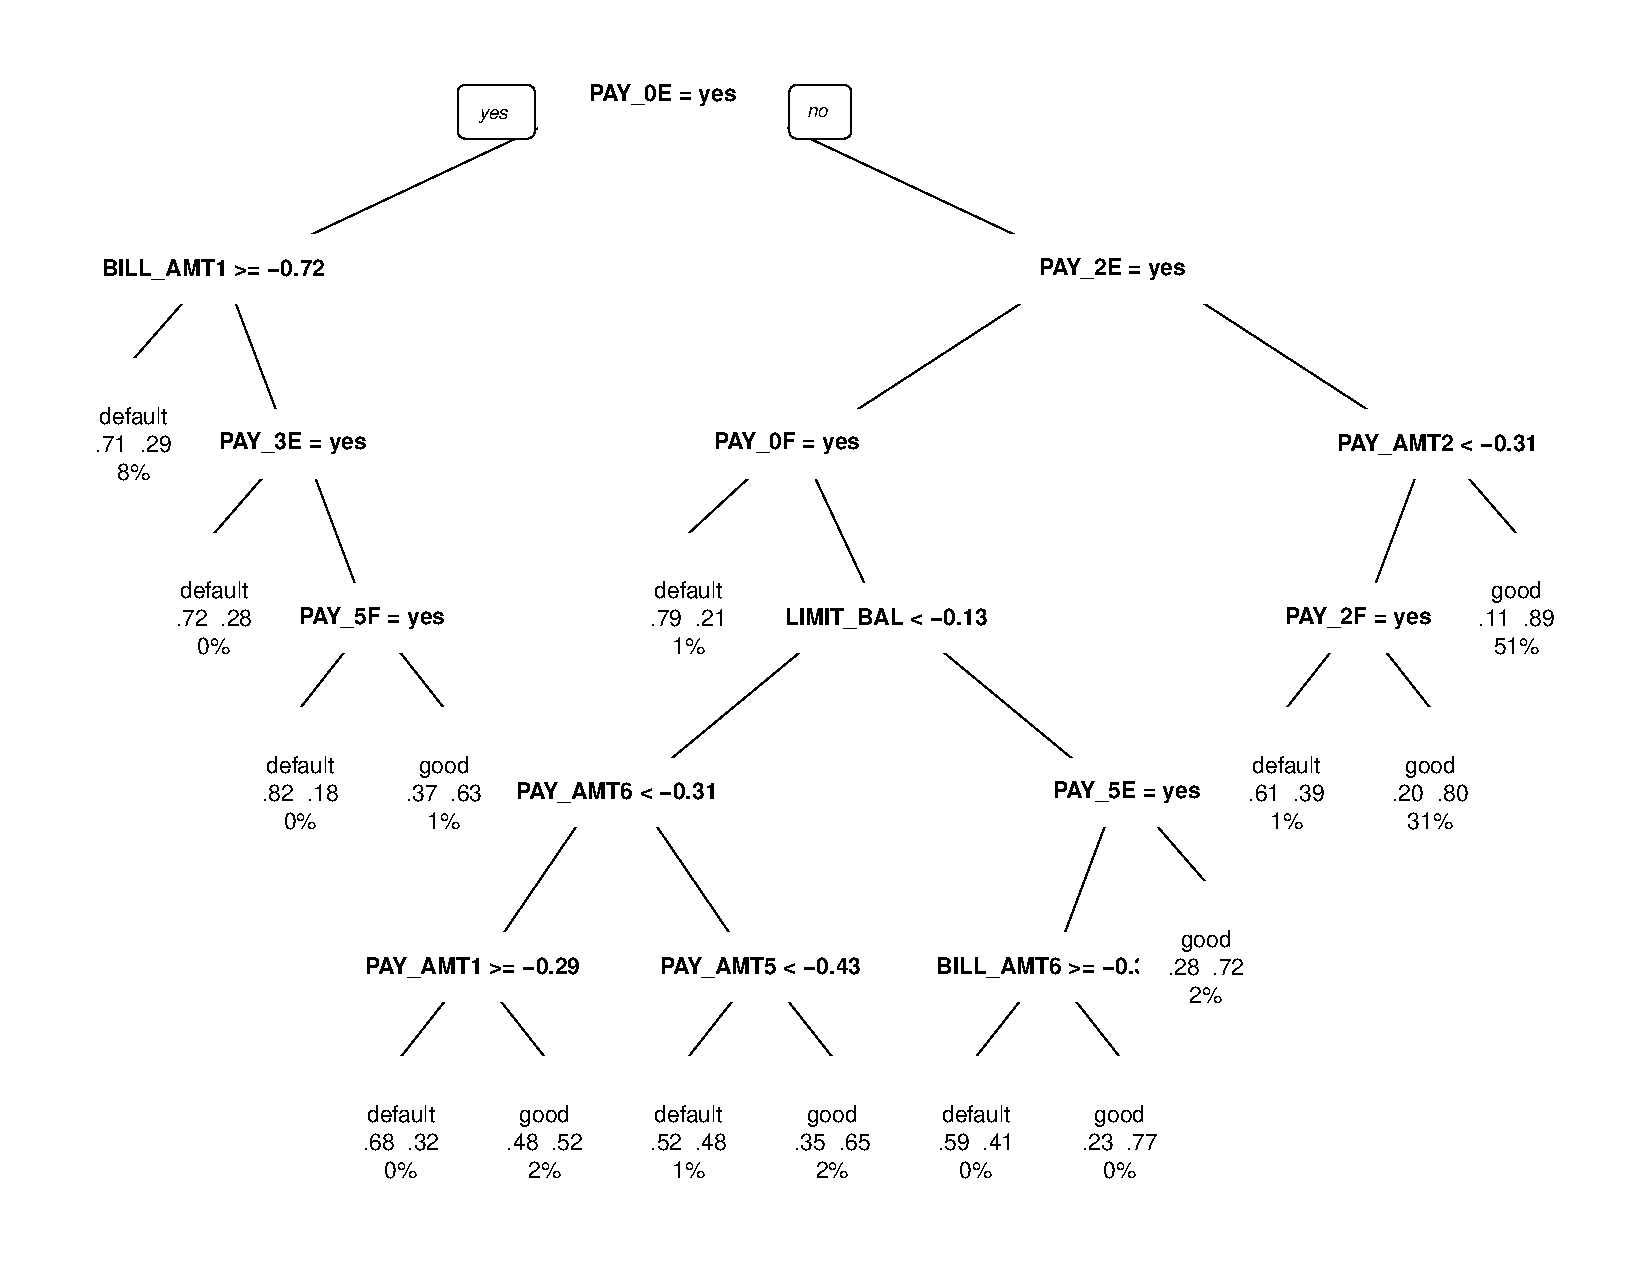
\includegraphics[width=5in]{Figures/DTsPlot.pdf} 
	\caption{Visualization of Decision Trees Model\protect\includegraphics[scale=0.1]{Figures/qletlogo.pdf}\href{https://github.com/Jingmin24/R-programming/tree/master/SPL_DecisionTreesModel}{SPL\_DecisionTreesModel}}\label{fig:dt} 
\end{figure}

From figure \ref{fig:dt}, we can interpret the process of decision trees model, for example, the test of variable in the root of the tree is whether the PAY\_0 (pay-situation in September) equals to ``E" (E represents -2), this variable is the most important explanatory variable for model`s prediction. In our case, 71\% of the samples is divided into ``default" class, when PAY\_0 equals to E and Bill\_ATM1 is bigger than -0.72.  
 \begin{center}
 	\begin{table}[!ht]
 		\centering  
 		\begin{tabular}{l|llc}
 			\hline\hline\\
 			& \multicolumn{2}{c}{Reference(DTs/RF)} \\		
 			Prediction & default   &    good \\			
 			\hline \\[-1.8ex] 			
 			default & 459 (475)    &   235 (234) \\ 					
 			good & 843 (827)    &   4284  (4285)\\ 			
 			\hline \hline			
 		\end{tabular}  
 		\caption{Confusion Matrix for Decision Trees and Random Forest Model} 	
 	\end{table}	
 \end{center}
Table 2 shows the confusion matrix of decision trees and random forest model, we can see that the confusion matrixes are similar for both, both model have higher accuracy in predicting ``good" class, with around 95\% of specificity., the difference is that the random forest has higher ability in predicting ``default" class.
 \begin{figure}[!ht] 
	\centering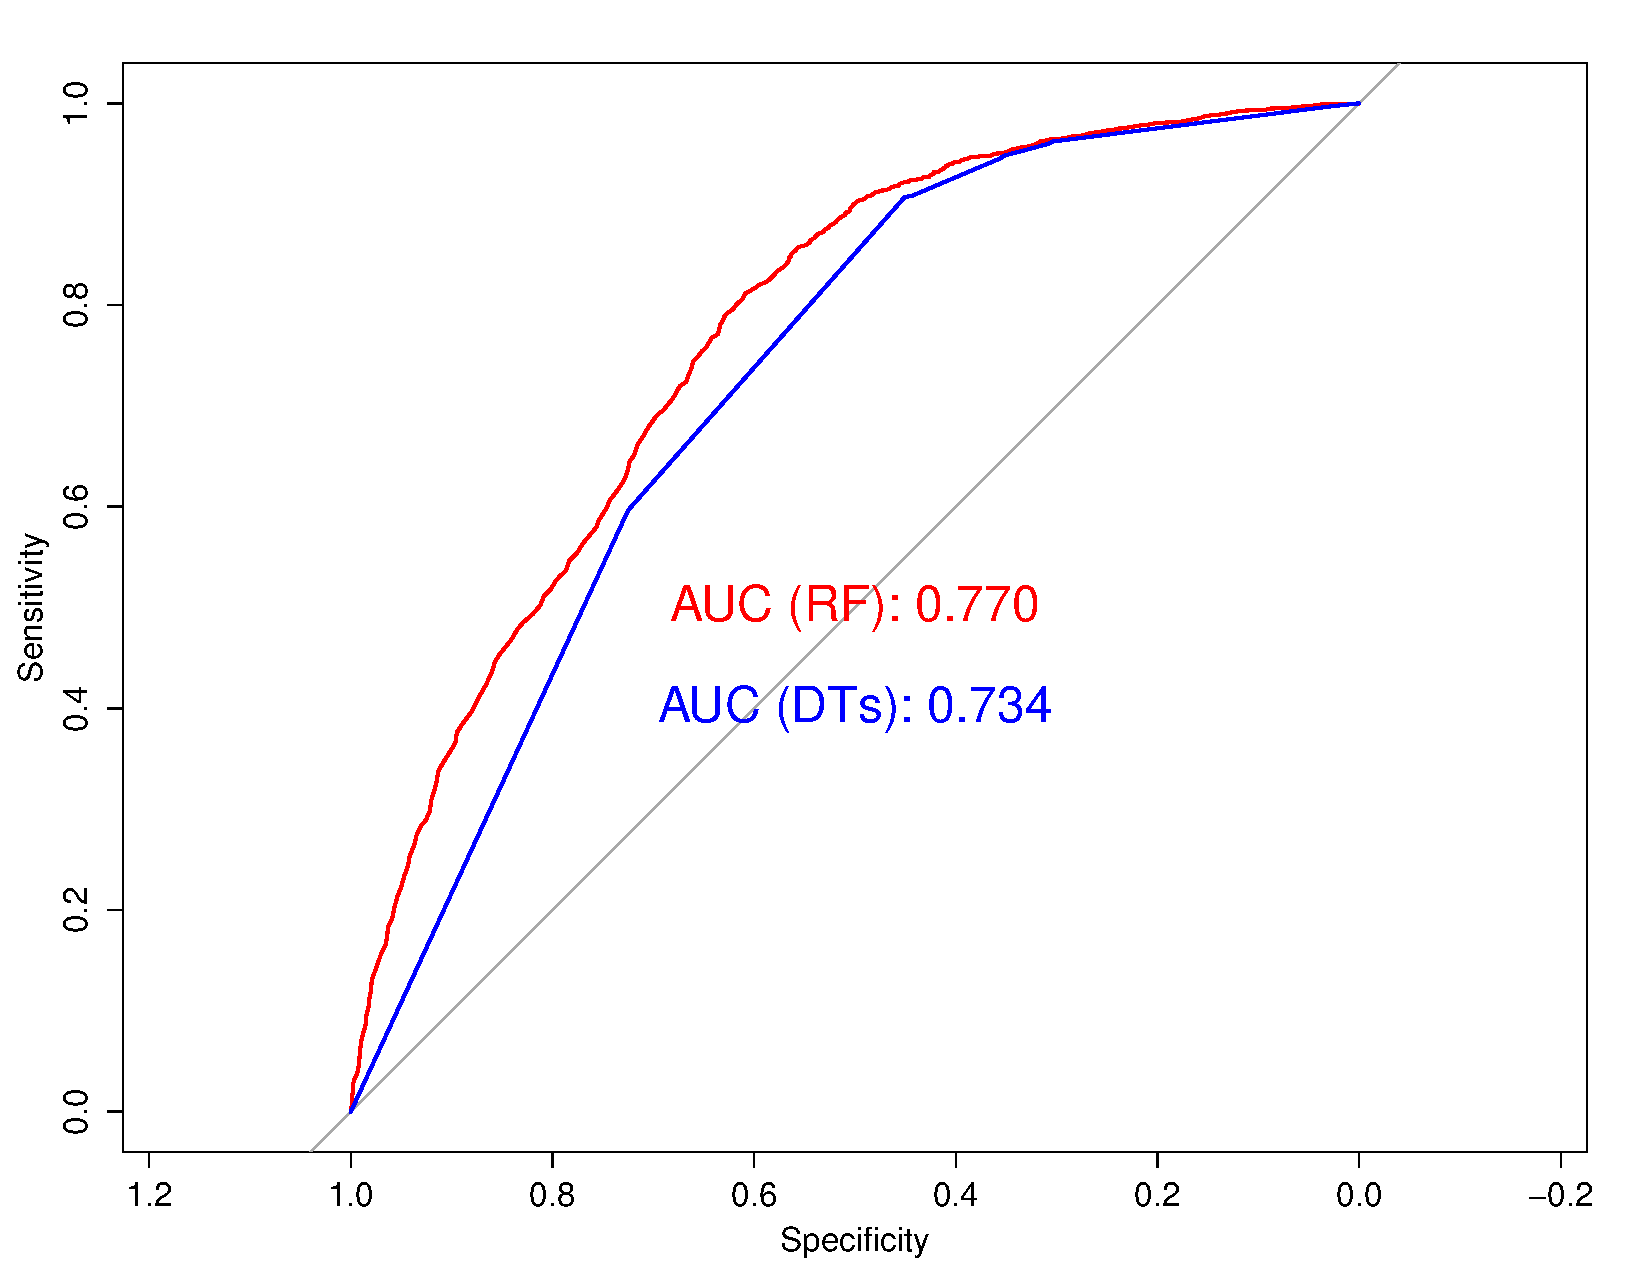
\includegraphics[width=4in]{Figures/AUCdtsrf.pdf} 
	\caption{ROC curves of DTs and RF\protect\includegraphics[scale=0.1]{Figures/qletlogo.pdf}\href{https://github.com/Jingmin24/R-programming/tree/master/SPL_RandomForest}{SPL\_RandomForest}}\label{fig:rocdtrf} 
\end{figure}

From Figure \ref{fig:rocdtrf}, we can see that random forest performs better than simple decision trees model, with higher AUC value (0.770 against 0.734).

However, the result suggests that both models have better performance in predicting the ``good" class and are less sensitive to ``default" class, the reason for this result may be that the data have unbalanced distribution of variable ``default\_payment\_next\_month", the number of ``good" class are almost 5 times higher than the ``default" class, so there are less information for the model to train.
\subsubsection{Logit Regresssion, Naive Bayes and Neural Network}
\begin{itemize}
	\item Input
\end{itemize}
The dataset we used is processed according to procedures explained as above, thus, we don not explaine agian here.
\begin{itemize}
	\item Actual output
\end{itemize}
One important result from the logistic regression is the significance of all independent variables (examples are shown in Table 3). As we can conclude in Table 3, the consumer whose education situation is ``others'', and the consumer who could not pay his credit debt duly in September would have high estimated probability of default in the next month. This result is explainable and easy to understand in practice, the consumer who could not pay his credit debt in this month has high probability of default payment in next month, because he may be already go bankrupt and this situation would continue. Comparing with these variables, some others are not very significant, which means they have less effects on the estimated probability of default.
\begin{table}[ht]
	\begin{center}
		{\footnotesize
			\begin{tabular}{l|cc}
				\hline \hline
				Independent Variables & Significance (***--very significant)& \\
				\hline
				Education-others  & ** \\
				Past payment in September-delay for one months & *  \\
				Past payment in September-delay for two months   &  *** \\
				Past payment in September-delay for three months    & ***  \\
				Past payment in September-delay for four months   &  *** \\
				Past payment in September-delay for five months  & ** \\
				\hline \hline
		\end{tabular}}
	\end{center}
	\caption{Siginificance of Independent Variables}
\end{table}

\begin{center}
	\begin{table}[!ht]
		\centering  
		\begin{tabular}{l|llc}
			\hline\hline\\
			& \multicolumn{2}{c}{Reference(NB/NN)} \\		
			Prediction & default   &    good \\			
			\hline \\[-1.8ex] 			
			default & 437 (842)    &   206 (455) \\ 					
			good & 856 (1239)    &   4305  (3267)\\ 			
			\hline \hline			
		\end{tabular}  
		\caption{Confusion Matrix for Naive Bayes Model and Neural Network } 	
	\end{table}	
\end{center}
From table 4, the accuracy can be computed easily by using equation as followings if we get confusion matrix:
\begin{equation}
	\left ( a+d\right )/\left ( a+b+c+d \right )=Accuracy
\end{equation}
where a, b, c and d represents four numbers in the confusion matrix.
Apparently, neural network((437+4305)/(437+206+856+4305)=0.817) has larger accuracy number than naive Bayes’((3267+842)/(842+455+1239+3267)=0.708), which proves neural network works better in our assignment and has more efficiency to predict the probability of default. About this argument, we get the same conclusion as the paper we simulated. 

 \begin{figure}[!ht] 
	\centering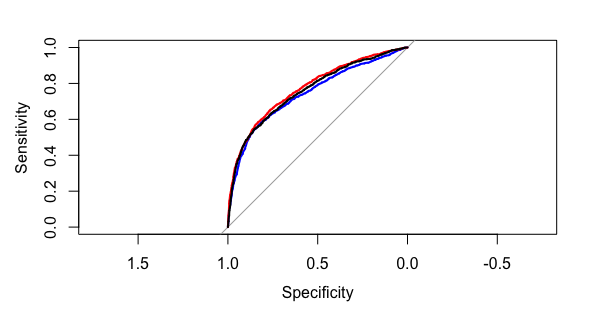
\includegraphics[width=4in,height=4in]{Figures/ROCALLN} 
	\caption{ROC curves of LR, NB and NN\protect\includegraphics[scale=0.1]{Figures/qletlogo.pdf}\href{https://github.com/Jingmin24/R-programming/blob/master/SPL_NeuralNetwork}{SPL\_NeuralNetwork}}\label{fig:ROCALLN} 
\end{figure}
From figure \ref{fig:ROCALLN}, three ROC lines almost overlap because of similar AUC numbers these models have, which can be obtained from the summary table 5.

\subsection{Model Evaluation}
\begin{table}[!htbp]
	\begin{center}
		\begin{tabular}{l|cccccc} 
			\hline\hline
			& LR & NB & NN & RF & DT\\ 
			\hline
			Acc & 0.8199 & 0.7085  & 0.8170 & 0.8225 & 0.8179  \\
			AUC & 0.7734  & 0.7442 & 0.7804 & 0.7701 & 0.7344\\
			\hline\hline
		\end{tabular}
		\caption{AUC and Accuracy results}
	\end{center}
\end{table}
Table 5 shows the results of AUC and accuracy for all the prediction models, we can see that with little difference in the number, the neural network model has the best performance, with 0.78 in AUC value. All models have an AUC value higher than 0.5, which is same with our expectation.

\newpage
\section{Conclusion}
This paper examines five different machine learning approaches on a dataset related to customer default payment of credit card in Taiwan, Credit risk control is very essential for a bank, the goal is to predict whether customers will default on the credit card payment or not in the future, the database is based on the information related to customer characteristics and some previous using situation of credit card.

In order to evaluate the performance of five prediction models, we use the area under the receiver operating characteristic curve (AUC) and accuracy value. The results indicate that there is little difference amount the prediction error rate among these models. However, when looking at the AUC value, there appear relatively large differences. The area ratio is a more suitable metric to measure the performance of models since it is more sensitive to the classification result to minority class of the data and in our project, the aimed variable ``default.payment.next month" has unbalanced distribution in two class. Our focus in this case is the minority class, which contains customers who default. The results show that the artificial neural network has the best performance with an AUC value of 0.78. Also, by comparing the results of logit regression and random forest, we find that attributes have different influence on different models. The demographic variables, like sex, education, are very important to predict the default risk in logit regression, but they have less influence in random forest model. However, information related to recent payment situation paly a big role in both two models, which suggests that the historical behavior somehow determines the future behavior of customers.

Further study should be related to testing the robustness of the prediction models using data in different time period, and improving the models by dealing with the problem of imbalanced distribution of response variable in dataset.

To sum up, the results of this paper show that we can use machine learning technology to analysis data and it is helpful to analysis and predict the behavior of customers. 

\newpage
\bibliography{reference}

\newpage
\section{Appendix}
SPL\_R-programming\\Github Page
\url{https://github.com/Jingmin24/R-programming.git}

\newpage
\section*{Declaration of Authorship}

We hereby confirm that we have authored this Seminar paper independently and without use of others than the indicated sources. All passages which are literally or in general matter taken out of publications or other sources are marked as such. 
\vspace{1cm}

Berlin, August 17, 2017 \vspace{0.5cm}

Jingmin Zhang, Yiying Zhang


\end{document}